\subsubsection{Klassifikation af KOLs sværhedsgrad}
Diagnosen af KOL vurderes på baggrund af patienters symptomer, egne erfaringer og livskvalitet. Dette vurderes ud fra Medical Research Council åndenødsskala (MRC) og COPD assessment test (CAT). Patienter kan efterfølgende inddeles i klassifikationer med udgangspunkt i MRC og CAT eller ved spirometrimålinger alene.\cite{Basisbogen2016}

 
MRC-skalaen er en skala fra $1$-$5$, hvor patienter vurderer mængden af aktivitet, som de kan udfører i forhold til åndenød. Skalaen fremgår af \autoref{fig:MRC}, hvor $1$ svarer til, at patienter først oplever åndenød ved meget anstrengelse, og $5$ svarer til, at patienter oplever åndenød ved meget lav fysisk aktivitet. \cite{Basisbogen2016}

\begin{figure} [H]
\centering
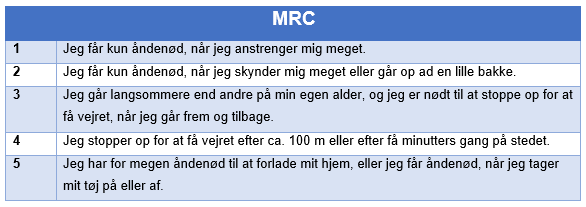
\includegraphics[width=0.9\textwidth]{figures/MRC}
\caption{MRC er en skala fra $1$-$5$. Patienter, der oplever åndenød ved meget anstrengelse vurderes som $1$, mens patienter der oplever åndenød ved lav aktivitet vurderes som $5$.}
\label{fig:MRC}
\end{figure} 

\noindent
En anden metode til at vurdere symptomerne ved KOL er  CAT-skema, hvor symptomerne vurderes fra $0$ til $5$. $0$ vurderes til, at patienter ingen symptomer har. Jo højere den samlede score er, desto værre vurderes patienters symptomer. Af \autoref{fig:CAT} ses CAT-skema til vurdering af symptomer.\cite{Basisbogen2016, dsam2016}

\begin{figure} [H]
\centering
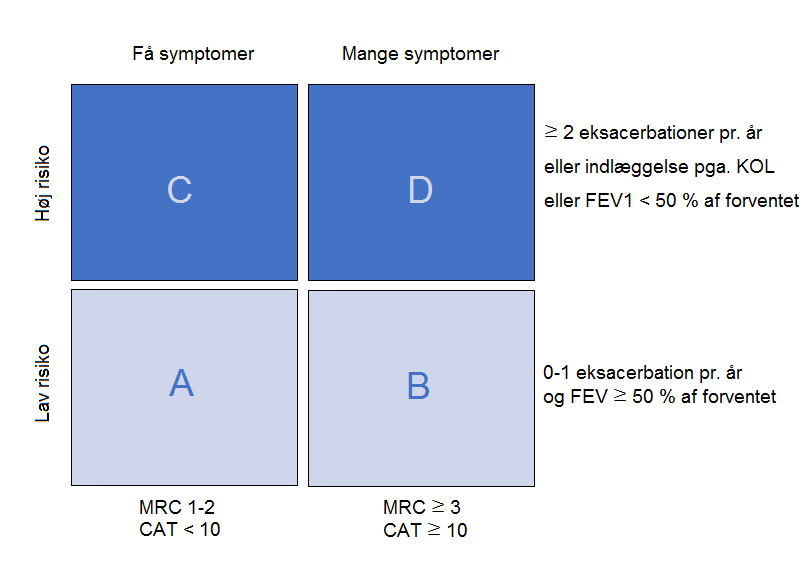
\includegraphics[width=0.9\textwidth]{figures/KAT}
\caption{*** MANGLER FIGUR** + TEKST}
\label{fig:CAT}
\end{figure} 



Ud fra MRC-skalaen eller CAT-skamet samt lungefunktionstest og antallet af eksacerbationer det seneste år kan KOL-patienter kategoriseres. Patienterne kategoriseres i fire forskellige kategorier; A, B, C og D, hvor D er patienter i høj risiko. Kategoriseringen fremgår af \autoref{fig:KAT}.

\begin{figure} [H]
\centering
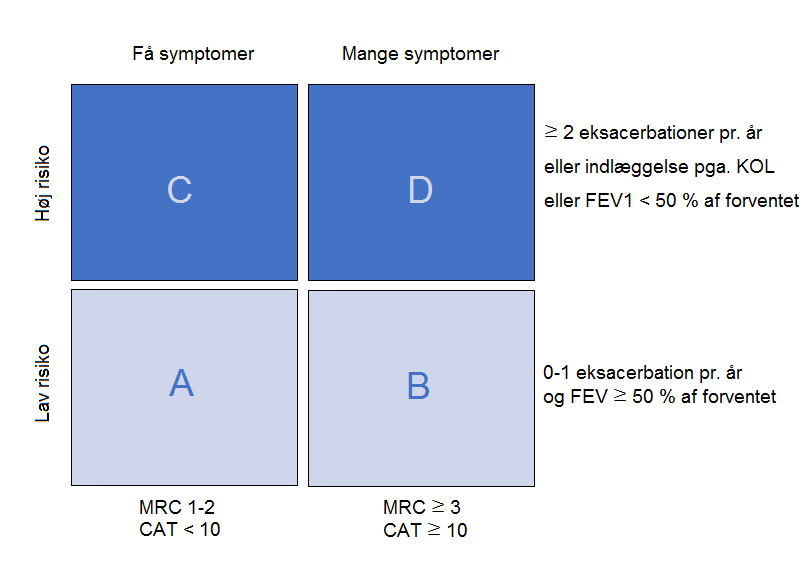
\includegraphics[width=0.8\textwidth]{figures/KAT}
\caption{KOL-patienter kategoriseres i fire kategorier herunder A, B, C og D. A og B inddeles i lav risiko, mens C og D er i høj risiko.}
\label{fig:KAT}
\end{figure} 
 
\noindent
Udover ABCD-kategoriseringen kan sværhedsgraden af KOL udelukkende bestemmes ud fra spiometrimålinger. Sværhedsgraden er klassificeret af Dansk Selskab for Almen Medicin (DSAM) ud fra retningslinjer opstillet af the Global Initiative for Chronic Obstructive Lung Disease (GOLD). Lungefunktion vurderes på baggrund af FEV$1$ i \% af den forventede lungekapacitet, hvoraf det inddeles i fire stadier. Disse fremgår af \autoref{fig:GOLD}.

\begin{figure} [H]
\centering
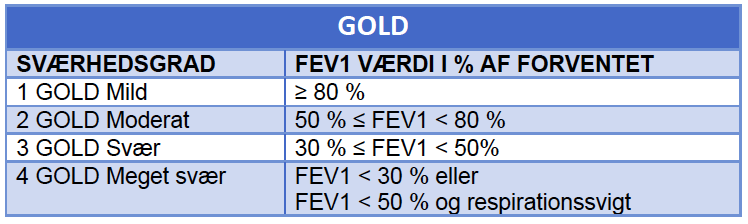
\includegraphics[width=0.8\textwidth]{figures/GOLD}
\caption{GOLD er inddelt efter sværhedsgraderne $1$-$4$ herunder mild, moderat, svær og meget svær. Patienter, der har over $80~\%$ af forventet lungekapacitet klassificeres som $1$ GOLD mild, mens patienter med under $30~\%$ eller over $50~\%$ af forventet lungekapacitet samt respirationssvigt, klassificeres som $4$ GOLD meget svær.}
\label{fig:GOLD}
\end{figure} 

\subsection{Behandling} \label{sec:behandling}
Da KOL er en kronisk lungesygdom er det ikke muligt at helbrede KOL-patienter. Dog er det muligt at bremse udviklingen af KOL samt lindre symptomerne, hvilket kan opnås ved tobakafvænning, fysisk aktivitet, kostvejledning og medicin. 

Da den tabte lungefunktionen ikke kan genvindes, rådes patienterne til tobakophør hurtigst muligt for således at bibeholde den nuværende lungefunktion. Det fremgår af \autoref{fig:fletcher}, hvordan tobak kan påvirke lungefunktionen over tid. 

\begin{figure} [H]
\centering
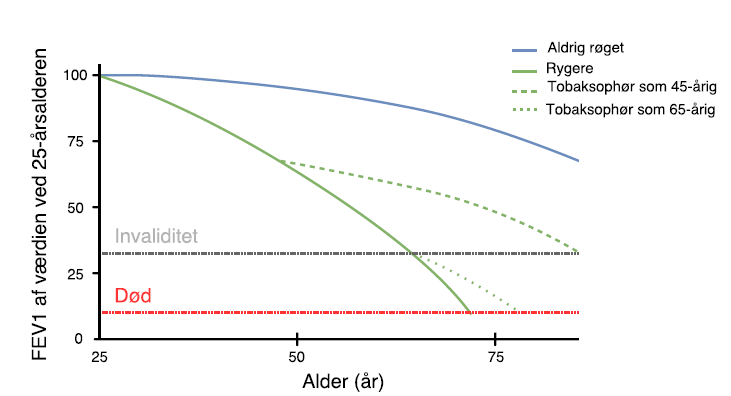
\includegraphics[width=0.5\textwidth]{figures/fletcher}
\caption{Fletcher-kurve, som viser faldet af FEV1 over tid for henholdsvis rygere, ikke-rygere og rygere med tobaksophør i $45$- og $65$-årsalderen.\cite{dsam2016}}
\label{fig:fletcher}
\end{figure} 

\noindent
Det ses af \autoref{fig:fletcher}, at tobak medvirker til et accelererende tab af FEV1, og dermed udsigt til kortere levetid. På trods af tobaksophør genoprettet FEV$1$ ikke, dog bremses accelerende tab af FEV$1$ til det normale aftag.\cite{dsam2016}

KOL-patienter med sekretproblemer tilbydes desuden continous positive airway pressure (CPAP) eller positive expiratory pressure (PEP-fløjte) og bronkodilaterende inhalationsbehandling efter behov og ud fra graden KOL. Yderligere kan antiinflammatorisk behandling gives til patienter med hyppige eksacerbationer. \cite{Basisbogen2016}
 
\subsection{Prognose}
KOL-patienter med eksacerbationer har efter indlæggelse en dødelighed på næsten $10$~$\%$ i løbet af den første måned. Dødeligheden ligger på omkring $64$ per $100.000$ per år for mænd og $54$ per $100.000$ per år for kvinder.
Udviklingen, hvormed sygdommen progredierer for KOL-patienter er specielt afhængig af, hvorvidt patienter ophører eksponering til den udløsende faktor for eksempel tobaksophør. Det er derfor vigtigt at få en tidlig diagnosticering således, at patienter hurtigt kan få hjælp. \cite{dsam2016}
%Derudover har et studie vist, at KOL-patienter, der er i stadie $4$ i GOLD-klassificeringen, har lav funktionalitet og livskvalitet, som bliver værre med tiden og ved fremkomst af flere symptomer til sygdommen. \cite{Habraken2011}

